\documentclass{../../../classes/anal}
\usepackage{pgfplots}
\pgfplotsset{compat=1.6}

\pgfplotsset{soldot/.style={color=blue,only marks,mark=*}}
\pgfplotsset{holdot/.style={color=blue,fill=white,only marks,mark=*}}

\title{Homework for week 1}

\begin{document}
    \section*{2.5}

    \problem{21}

    \begin{equation}
        \begin{aligned}
            \lim_{x\to 2^-}f(x) &\neq \lim_{x\to 2^+}f(x) & \implies \\
            \lim_{x\to 2^-}(x + 3) &\neq \lim_{x\to 2^+}2^x & \implies \\
            \lim_{x\to 2^-}x + \lim_{x\to 2^-}3 &\neq \lim_{x\to 2^+}2^x & \implies \\
            2 + 3 &\neq 2^2
        \end{aligned}
    \end{equation}

    \begin{tikzpicture}
        \begin{axis}[xmin=-3,xmax=3,ymin=-1,ymax=4]
            \addplot[domain=-3:-1,blue,samples=100] {x+3};
            \addplot[domain=-1:3,blue,samples=100] {2^x};
            \addplot[holdot,blue,fill=white] coordinates{(-1,1/2)};
            \addplot[soldot,blue] coordinates{(-1,2)};
        \end{axis}
    \end{tikzpicture}

    \problem{23}

    \begin{equation}
        \begin{aligned}
            \lim_{x\to 0}f(x) &\neq f(0) & \implies \\
            \lim_{x\to 0}(1 - x^2) &\neq 0 & \implies \\
            \lim_{x\to 0}1 + \lim_{x\to 0}x^2 &\neq 0 & \implies \\
            1 + 0 &\neq 0
        \end{aligned}
    \end{equation}

    \begin{tikzpicture}
        \begin{axis}[xmin=-3,xmax=3,ymin=-2,ymax=3]
            \addplot[domain=-3:0,blue,samples=100] {cos(deg(x))};
            \addplot[domain=0:3,blue,samples=100] {1-x^2};
            \addplot[holdot,blue,fill=white] coordinates{(0,1)};
            \addplot[soldot,blue] coordinates{(0,0)};
        \end{axis}
    \end{tikzpicture}

    \problem{25}

    \begin{enumerate}[label={(\alph*)}]
        \item {since \(\lim_{x\to3}f(x)\) exists and is equal to \({1 \over 6}\) but \(f(3)\) doesn't exist, the discontinuity is removable.}
        \item {\[f(x) = \begin{cases}
            {x - 3 \over x^2 - 9} & \text{if} \ x \neq 3 \\
            {1 \over 6} & \text{if} \ x = 3 \\
        \end{cases}\]}
    \end{enumerate}

    \problem{43}

    \(f(x)\) is discontinuous but continuous from the right at \(x=-1\).

    \begin{tikzpicture}
        \begin{axis}[xmin=-3,xmax=3,ymin=-2,ymax=3]
            \addplot[domain=-3:-1,blue,samples=100] {x^2};
            \addplot[domain=-1:1,blue,samples=100] {x};
            \addplot[domain=1:3,blue,samples=100] {1/x};
            \addplot[holdot,blue,fill=white] coordinates{(-1,1)};
            \addplot[soldot,blue] coordinates{(-1,-1)(1,1)};
        \end{axis}
    \end{tikzpicture}

    \problem{48}

    \begin{equation*}
        f(x) = \begin{cases}
            {x^2 - 4 \over x - 2} & \text{if} \ x < 2 \\
            {ax^2 - bx + 3} & \text{if} \ 2 \leq x < 3 \\
            {2x - a + b} & \text{if} \ 3 \leq x 
        \end{cases}
    \end{equation*}
    
    we know that $\lim_{x\to2^+}f(2) = f(2)$ and $\lim_{x\to3^+}f(x) = f(3)$, so all that's left to align are $\lim_{x\to2^-}f(x) = f(2)$ and $\lim_{x\to3^-}f(x) = f(3)$

    \begin{equation}
        \begin{aligned}
            \lim_{x\to2^-}f(x) 
            &= \lim_{x\to2^-}{x^2 - 4 \over x - 2} \\ 
            &= \lim_{x\to2^-}{(x - 2)(x + 2) \over x - 2} \\ 
            &= \lim_{x\to2^-}{(x + 2)} \\ 
            &= 4
        \end{aligned}
    \end{equation}

    \begin{equation}
        \begin{aligned}
            f(2) 
            &= a\cdot2^2-b\cdot2+3 \\
            &= 4a - 2b + 3
        \end{aligned}
    \end{equation}

    \begin{equation} \label{eq:p48:1}
        \lim_{x\to2^-}f(x) = f(2) \implies 4 = 4a - 2b + 3 \implies 4a - 2b = 1
    \end{equation}

    and

    \begin{equation}
        \begin{aligned}
            \lim_{x\to3^-}f(x)  
            &= \lim_{x\to3^-}(ax^2 - bx + 3) \\
            &= 9a - 3b + 3
        \end{aligned}
    \end{equation}

    \begin{equation}
        \begin{aligned}
            f(3)
            &= 2\cdot3 - a + b \\
            &= 6 - a + b
        \end{aligned}
    \end{equation}

    \begin{equation} \label{eq:p48:2}
        \lim_{x\to3^-}f(x)
        = f(3)
        \implies
        9a - 3b + 3
        = 6 - a + b
        \implies
        10a - 4b = 3
    \end{equation}
    
    then, we simply have the following system to solve:

    \begin{equation}
        \begin{aligned}
            &\begin{cases}
                10a - 4b = 3 & \eqref{eq:p48:1} \\
                4a - 2b = 1 & \eqref{eq:p48:2}
            \end{cases}
            \\ \implies
            &\begin{cases}
                10a - 4b = 3 \\
                -8a + 4b = -2
            \end{cases}
            \\ \implies
            &\begin{cases}
                2a = 1 \\
                4({1 \over 2}) - 2b = 3
            \end{cases}
            \\ \implies
            &\begin{cases}
                2a = 1 \\
                2b = 1
            \end{cases}
            \\ \implies
            &\begin{cases}
                a = {1 \over 2} \\
                b = {1 \over 2}
            \end{cases}
        \end{aligned}
    \end{equation}

    the corresponding graph:

    \begin{tikzpicture}
        \begin{axis}[xmin=1,xmax=4]
            \addplot[domain=0:2,blue,samples=100] {(x^2-4)/(x-2)};
            \addplot[domain=2:3,blue,samples=100] {0.5*x^2-0.5*x+3};
            \addplot[domain=3:5,blue,samples=100] {2*x-0.5+0.5};
            \addplot[holdot,blue,fill=white] coordinates{(2,4)(3,9*0.5-3*0.5+3)};
            \addplot[soldot,blue] coordinates{(2,4*0.5-2*0.5+3)(3,6)};
        \end{axis}
    \end{tikzpicture}

    \problem{55}

    Given that \(f(x) = -x^3 + 4x + 1\) is continuous and the range \((-1, 0)\) maps to \((-2, 1)\), by the Intermediate Value Theorem we know that if \(f(a) = 0\) then \(a \in (-1, 0)\).

    \problem{72}

    \(f(x)\) is never continuous.

    \section*{2.6}

    \problem{3}

    \begin{enumerate}[label={(\alph*)}]
        \item \(\lim_{x\to\infty}f(x) = -2\)
        \item \(\lim_{x\to-\infty}f(x) = 2\)
        \item \(\lim_{x\to1}f(x) = \infty\)
        \item \(\lim_{x\to3}f(x) = -\infty\)
        \item \begin{itemize}
            \item \(y = 2\)
            \item \(y = -2\)
            \item \(x = 1\)
            \item \(x = 3\)
        \end{itemize}
    \end{enumerate}

    \problem{5}

    \begin{tikzpicture}
        \begin{axis}[xmin=-4,xmax=4]
            \addplot[domain=-4:-2,blue,samples=100]{(4*(-10*(x+1.9))-2)/(-(-10*(x+1.9))^2)};
            \addplot[domain=-2:2,blue,samples=100] {x};
            \addplot[domain=2:4,blue,samples=100]  {(2*(20*x+0.5-40)-1)/(20*x+5-40)^2+2};
            \addplot[red] {0};
            \addplot[red] {2};
        \end{axis}
    \end{tikzpicture}

    \problem{9}

    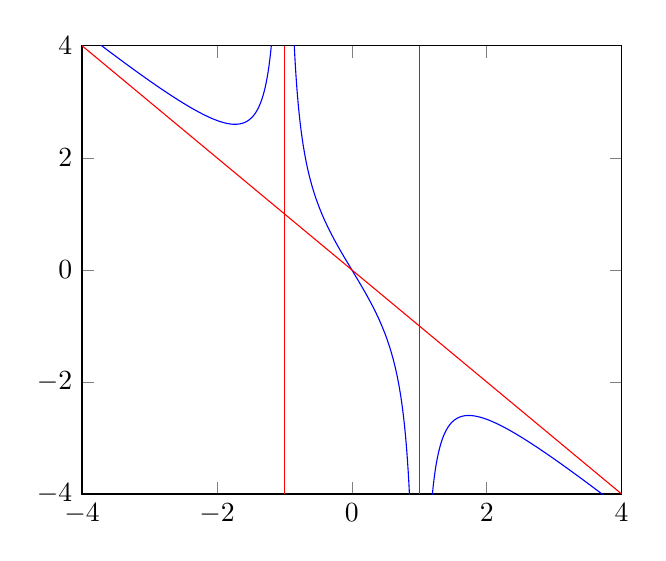
\begin{tikzpicture}
        \begin{axis}[xmin=-4,xmax=4,ymin=-4,ymax=4]
            \addplot[blue,samples=1000]{-x*abs(x+1)*abs(x-1)/((x-1)*(x+1)*(x-1)*(x+1))-x};
            \addplot[red] coordinates{(-1,4)(-1,-4)};
            \addplot[red] coordinates{(1,4)(1,-4)};
            \addplot[red] coordinates{(-4,4)(4,-4)};
            % \addplot[red] {x=-1};
        \end{axis}
    \end{tikzpicture}

    \problem{13}

    \begin{equation*}
        \begin{aligned}
            \lim_{x\to\infty} {2x^2 -7 \over 5x^2 + x - 3}
            &= \lim_{x\to\infty} {{2x^2 -7 \over x^2} \over {5x^2 + x - 3 \over x^2}}
            = \lim_{x\to\infty} {2 - {7 \over x^2} \over 5 + {1 \over x} - {3 \over x^2}} \\
            &= {\lim_{x\to\infty} \left(2 - {7 \over x^2}\right) \over \lim_{x\to\infty} \left(5 + {1 \over x} - {3 \over x^2}\right)} & \text{(by Limit Law 5)}\\
            &= {\lim_{x\to\infty} 2 - \lim_{x\to\infty}{7 \over x^2} \over \lim_{x\to\infty} 5 + \lim_{x\to\infty} {1 \over x} - \lim_{x\to\infty}{3 \over x^2}} &\text{(by 1, 2 and 3)} \\
            &= {2 - 0 \over 5 + 0 - 0} & \text{(by 8 and Theorem 5)} \\
            &= {2 \over 5}
        \end{aligned}
    \end{equation*}

    \problem{17}

    \begin{equation*}
        \begin{aligned}
            \lim_{t\to-\infty} {3t^2 + t \over t^2 - 4t + 1}
            &= \lim_{t\to-\infty} {{3t^2 + t \over t^2} \over {t^2 - 4t + 1 \over t^2}}
            = \lim_{t\to-\infty} {3 + {1 \over t} \over 1 - {4 \over t} + {1 \over t^2}} \\
            &= {\lim_{t\to-\infty}\left(3 + {1 \over t}\right) \over \lim_{t\to-\infty}\left(1 - {4 \over t} + {1 \over t^2}\right)} \\
            &= {\lim_{t\to-\infty}3 + \lim_{t\to-\infty}{1 \over t} \over \lim_{t\to-\infty}1 - \lim_{t\to-\infty}{4 \over t} + \lim_{t\to-\infty}{1 \over t^2}} \\
            &= {3 + 0 \over 1 - 0 + 0} \\
            &= 3
        \end{aligned}
    \end{equation*}

    \problem{23}

    \begin{equation*}
        \begin{aligned}
            \lim_{x\to\infty} {\sqrt{x + 3x^2} \over 4x - 1}
            &= \lim_{x\to\infty} {\sqrt{{1 \over x} + 3} \over 4 - {1 \over x}} \\
            &= {\lim_{x\to\infty} \sqrt{{1 \over x} + 3} \over \lim_{x\to\infty} \left(4 - {1 \over x}\right)} \\
            &= {\sqrt{\lim_{x\to\infty}{1 \over x} + \lim_{x\to\infty}3} \over \lim_{x\to\infty}4 - \lim_{x\to\infty}{1 \over x}} \\
            &= {\sqrt{0 + 3} \over 4 - 0} \\
            &= {\sqrt{3} \over 4} \\
        \end{aligned}
    \end{equation*}

    \problem{29}

    \begin{equation*}
        \begin{aligned}
            \lim_{t\to\infty} \left(\sqrt{25t^2 + 2} - 5t\right)
            &= \lim_{t\to\infty} t{\sqrt{25t^2 + 2} - 5t \over t} \\
            &= \lim_{t\to\infty} t\left(\sqrt{25 + {2 \over t}} - 5\right) \\
            &= (\lim_{t\to\infty} t) \cdot \left(\lim_{t\to\infty}\sqrt{25 + {2 \over t}} - \lim_{t\to\infty}5\right) \\
            &= (\lim_{t\to\infty} t) \cdot \left(\sqrt{\lim_{t\to\infty}25 + \lim_{t\to\infty}{2 \over t}} - \lim_{t\to\infty}5\right) \\
            &= \infty \cdot \left(\sqrt{25 + 0} - 5\right) \\
            &= 0 \\
        \end{aligned}
    \end{equation*}

    \problem{33}

    \begin{equation*}
        \begin{aligned}
            \lim_{x\to-\infty} \left(x^2 + 2x^7\right)
            &= \lim_{x\to-\infty} x^7\left({1 \over x^5} + 2\right) \\
            &= \lim_{x\to-\infty} x^7 \cdot \lim_{x\to-\infty} \left({1 \over x^5} + 2\right) \\
            &= -\infty
        \end{aligned}
    \end{equation*}

    \problem{37}

    \begin{equation*}
        \begin{aligned}
            \lim_{x\to\infty}{1 - e^x \over 1 + 2e^x}
            &= \lim_{x\to\infty}{{1 - e^x \over e^x} \over {1 + 2e^x \over e^x}} \\
            &= \lim_{x\to\infty}{{1 \over e^x} - 1 \over {1 \over e^x} + 2} \\
            &= {\lim_{x\to\infty}{1 \over e^x} - \lim_{x\to\infty} 1 \over \lim_{x\to\infty} {1 \over e^x} + \lim_{x\to\infty} 2} \\
            &= {0 - 1 \over 0 + 2} \\
            &= -{1 \over 2}
        \end{aligned}
    \end{equation*}

    \problem{41}

    \begin{equation*}
        \begin{aligned}
            \lim_{x\to\infty}\left[\ln(1 + x^2) - \ln(1 + x)\right]
            &= \lim_{x\to\infty}\ln\left({1 + x^2 \over 1 + x}\right) \\
            &= \ln\left(\lim_{x\to\infty}{1 + x^2 \over 1 + x}\right) \\
            &= \ln\left(\lim_{x\to\infty}{{1 \over x^2} + 1 \over {1 \over x^2} + {1 \over x}}\right) \\
            &= \ln\left(\infty\right) \\
            &= \infty
        \end{aligned}
    \end{equation*}

    \problem{47}

    asymptotes: \(x = -3, y = 4\)

    \problem{49}

    asymptotes: \(x = -2, x = 1, y = 2\)

    \problem{61}

    \begin{equation}
        \begin{aligned}
            \lim_{x\to\infty} \left(x^4 - x^6\right)
            &= \lim_{x\to\infty} x^6\left({1 \over x^2} - 1\right) \\
            &= (\lim_{x\to\infty} x^6) \cdot \lim_{x\to\infty}\left({1 \over x^2} - 1\right) \\
            &= (\lim_{x\to\infty} x^6) \cdot \left(\lim_{x\to\infty}{1 \over x^2} - \lim_{x\to\infty}1\right) \\
            &= \infty \cdot \left(0 - 1\right) \\
            &= -\infty \\
        \end{aligned}
    \end{equation}

    \problem{65}

    \begin{enumerate}[label={(\alph*)}]
        \item {
            \(f(x) = {\sin x \over x}\). Let \(g(x) = -{1 \over |x|}\) and \(h(x) = {1 \over |x|}\). It's clear that \(g(x) \leq f(x) \leq h(x)\). Since \(\lim_{x\to\infty}g(x) = \lim_{x\to\infty}h(x)\), by the Squeeze Theorem, we can say that \(\lim_{x\to\infty}f(x) = \lim_{x\to\infty}g(x) = \lim_{x\to\infty}h(x)\). 

            \begin{equation}
                \begin{aligned}
                    \lim_{x\to\infty}f(x)
                    &= \lim_{x\to\infty}h(x) \\
                    &= \lim_{x\to\infty}{1 \over |x|} \\
                    &= 0 \\
                \end{aligned}
            \end{equation}
        }
        \item {
            \begin{tikzpicture}
                \begin{axis}[xmin=-2,xmax=100,ymin=-1.2,ymax=1.2]
                    \addplot[domain=-2:100,blue,samples=1000] {sin(deg(x))/x};
                    \addplot[domain=-2:100,red,samples=10] {0};
                \end{axis}
            \end{tikzpicture}

            the function crosses it's asymptote infinitely many times.
        }
    \end{enumerate}

    \problem{57}

    \[f(x) = \frac{1}{-\left|x\right|}+\frac{1}{3-x}-\frac{1}{\left(x-2\right)^{2}+2}\]

    \section*{2.7}

    \problem{3}

    \begin{enumerate}[label={(\alph*)}]
        \item \begin{enumerate}[label={(\roman*)}]
            \item \begin{equation*}
                \begin{aligned}
                    m 
                    &= \lim_{x\to-1} {f(x) - f(-1) \over x + 1} \\
                    &= \lim_{x\to-1} {(x^2 + 3x) - ((-1)^2 + 3(-1)) \over x + 1} \\
                    &= \lim_{x\to-1} {x^2 + 3x + 2 \over x + 1} \\
                    &= \lim_{x\to-1} {(x + 1)(x + 2) \over x + 1} \\
                    &= \lim_{x\to-1} (x + 2) \\
                    &= 1
                \end{aligned}
            \end{equation*}
            \item \begin{equation*}
                \begin{aligned}
                    m
                    &= \lim_{h\to0} {f(-1 + h) - f(-1) \over h} \\ 
                    &= \lim_{h\to0} {((-1 + h)^2 + 3(-1 + h)) - ((-1)^2 + 3(-1)) \over h} \\ 
                    &= \lim_{h\to0} {(1 - 2h + h^2 - 3 + 3h) - (1 - 3) \over h} \\ 
                    &= \lim_{h\to0} {1 - 2h + h^2 - 3 + 3h + 2 \over h} \\ 
                    &= \lim_{h\to0} {h + h^2 \over h} \\ 
                    &= \lim_{h\to0} 1 + h \\ 
                    &= 1 \\ 
                \end{aligned}
            \end{equation*}
        \end{enumerate}
        \item \(y = x - 1\)
    \end{enumerate}

    \problem{7}

    \begin{equation*}
        \begin{aligned}
            m 
            &= \lim_{h\to0} {f(2 + h) - f(2) \over h} \\
            &= \lim_{h\to0} {{2 + h + 2 \over 2 + h - 3} - {2 + 2 \over 2 - 3} \over h} \\
            &= \lim_{h\to0} {{4 + h \over h - 1} + 4 \over h} \\
            &= \lim_{h\to0} {4 + h + 4h - 4 \over h(h - 1)} \\
            &= \lim_{h\to0} {5h \over h(h - 1)} \\
            &= \lim_{h\to0} {5 \over (h - 1)} \\
            &= {5 \over (0 - 1)} \\
            &= -5 \\
        \end{aligned}
    \end{equation*}

    \problem{11}

    \begin{enumerate}[label={(\alph*)}]
        \item \begin{equation*}
            \begin{aligned}    
                4.9t^2 &= 30 & \implies \\
                t^2 &= {30 \over 4.9} & \implies \\
                t &= \sqrt{30 \over 4.9} = {10\sqrt{3} \over 7}
            \end{aligned}
        \end{equation*}
        \item \begin{equation*}
            \begin{aligned}
                v
                &= \lim_{h\to0} {4.9\left({10\sqrt{3} \over 7} + h\right)^2 - 4.9\left({10\sqrt{3} \over 7}\right)^2 \over h} \\
                &= \lim_{h\to0} {4.9\left({300 \over 49} + 2h{10\sqrt{3} \over 7} + h^2\right) - 4.9\left({300 \over 49}\right) \over h} \\
                &= \lim_{h\to0} {30 + 4.9 \cdot 2h{10\sqrt{3} \over 7} + 4.9 h^2 - 30 \over h} \\
                &= 4.9 \cdot \lim_{h\to0} {2h{10\sqrt{3} \over 7} + h^2 \over h} \\
                &= 4.9 \cdot \lim_{h\to0} \left(2{10\sqrt{3} \over 7} + h\right) \\
                &= 14\sqrt{3} \\
            \end{aligned}
        \end{equation*}
    \end{enumerate}

    \problem{15}

    \begin{enumerate}[label={(\alph*)}]
        \item The particle is moving to the right during time intervals \([0, 1]\) and \([4, 6]\). It's moving to the left during time interval \([2, 3]\). It's standing still during \([1, 2]\) and \([3, 4]\).
        \item \begin{tikzpicture}
            \begin{axis}[]
                \addplot[domain=0:1,blue] {3};
                \addplot[domain=1:2,blue] {0};
                \addplot[domain=2:3,blue] {-2};
                \addplot[domain=3:4,blue] {0};
                \addplot[domain=4:6,blue] {1};
            \end{axis}
        \end{tikzpicture}
    \end{enumerate}
\end{document}